%*******************************************************************************
%*********************************** Fourth Chapter *****************************
%*******************************************************************************

\chapter{Molecule VR Viewer- implementation}\label{chapter4}  %Title of the Fourth Chapter

As previous chapter outlines the result of this work, it does not provide description of methodology needed for creating Molecule VR Viewer. Therefore, this chapter is devoted to programming details, used algorithms and implementation of the project.

%********************************** %First Section  **************************************
\section{\textit{Unity 3D}} %Section - 4.1 

\textit{Unity 3D} game engine provides IDE (Integrated Development Environment) for games and other interactive materials, both in 2D and 3D. In version 5.3, itt enables writing scripts in two languages: UnityScript and C\#. The latter one was used for this work's purpose.

For better understanding of Molecule VR Viewer implementation, the following subsections describe the components needed for creating  materials in \textit{Unity 3D} and explain how do they work.

\subsection{Editor}

Generally saying, \textit{Unity 3D} products are created on two tracks: Editor and Scripting. The first one is editable in main window of application, showing the scenes of the project, their environments and objects.

Objects in \textit{Unity 3D}, called GameObjects, are containers that hold Components and Scripts, which may influence their apperance, properties and actions. For example, every GameObject has the Transform Component, which represents position and orientation i space. The engine serves a huge variety of editable Components, which may be attached to the object, like its physical properties, its material etc. Moreover, some of the general GameObject types containing needed Components are provided by \textit{Unity 3D}, e.g. Cameras, which are responsible for observing the scene, Lights, 3D basic models, UI (User's Interface) elements etc. Additionally, the GameObjects can be stored as templates called Prefabs, from which one can create new instances of the GameObject \cite{Unity16}.

Summing up, Editor mode is the core of the whole project, which enables the developer to combine all of the needed objects, create Scenes, change player settings (like enabling Unity VR Support) and manage it all to create the final product.


\subsection{Scripting}

The second track of developing programs in \textit{Unity 3D} is Scripting. Scripts may be responsible for arranging events and responds in the Gameplay mode, they can influence Components of GameObjects, create and destroy GameObjects etc. As they play huge role in whole mechanism of game or material creating, it is worth knowing their manner of working.

First of all, \textit{Unity} scripts derive from the built-in class MonoBehaviour, which is the base class connecting the script with internal workings of \textit{Unity} engine. By default, the script defines two methods: Start, which is responsible for all initialisations before the gameplay begins, and the next one, Update, which is the place for code that is going to be called once per frame during the gameplay. 

Secondly, it is worth mentioning, that scripts created for \textit{Unity} do not contain constructor functions. This feature is supported by the Editor mode, when script is attached to some GameObject as its Component, which is equal to creating an instance of the class. What is more, variables declared in the class field, which are public, are editable in Editor mode and can be even linked with another GameObject.

Thirdly, scripts are able to access other components that belong to the same GameObject or even to different GameObjects \cite{Unity16}. 

\subsubsection{Event Functions}

Start and Update functions mentioned above are in fact just two examples of the big group of event functions, which are activated  in certain moments of a gameplay. They are the consequence of the fact, that \textit{Unity} does not run the code continuously, script by script. Instead, scripts take control intermittently, when their certain functions are called by \textit{Unity}. After the function's execution, control is passed back to the engine \cite{Unity16}. 

The remaining examples of event functions and their order of execution are shown on the flowchart in Figure \ref{fig:monobehaviour}.

\begin{figure}[p]
\centering    
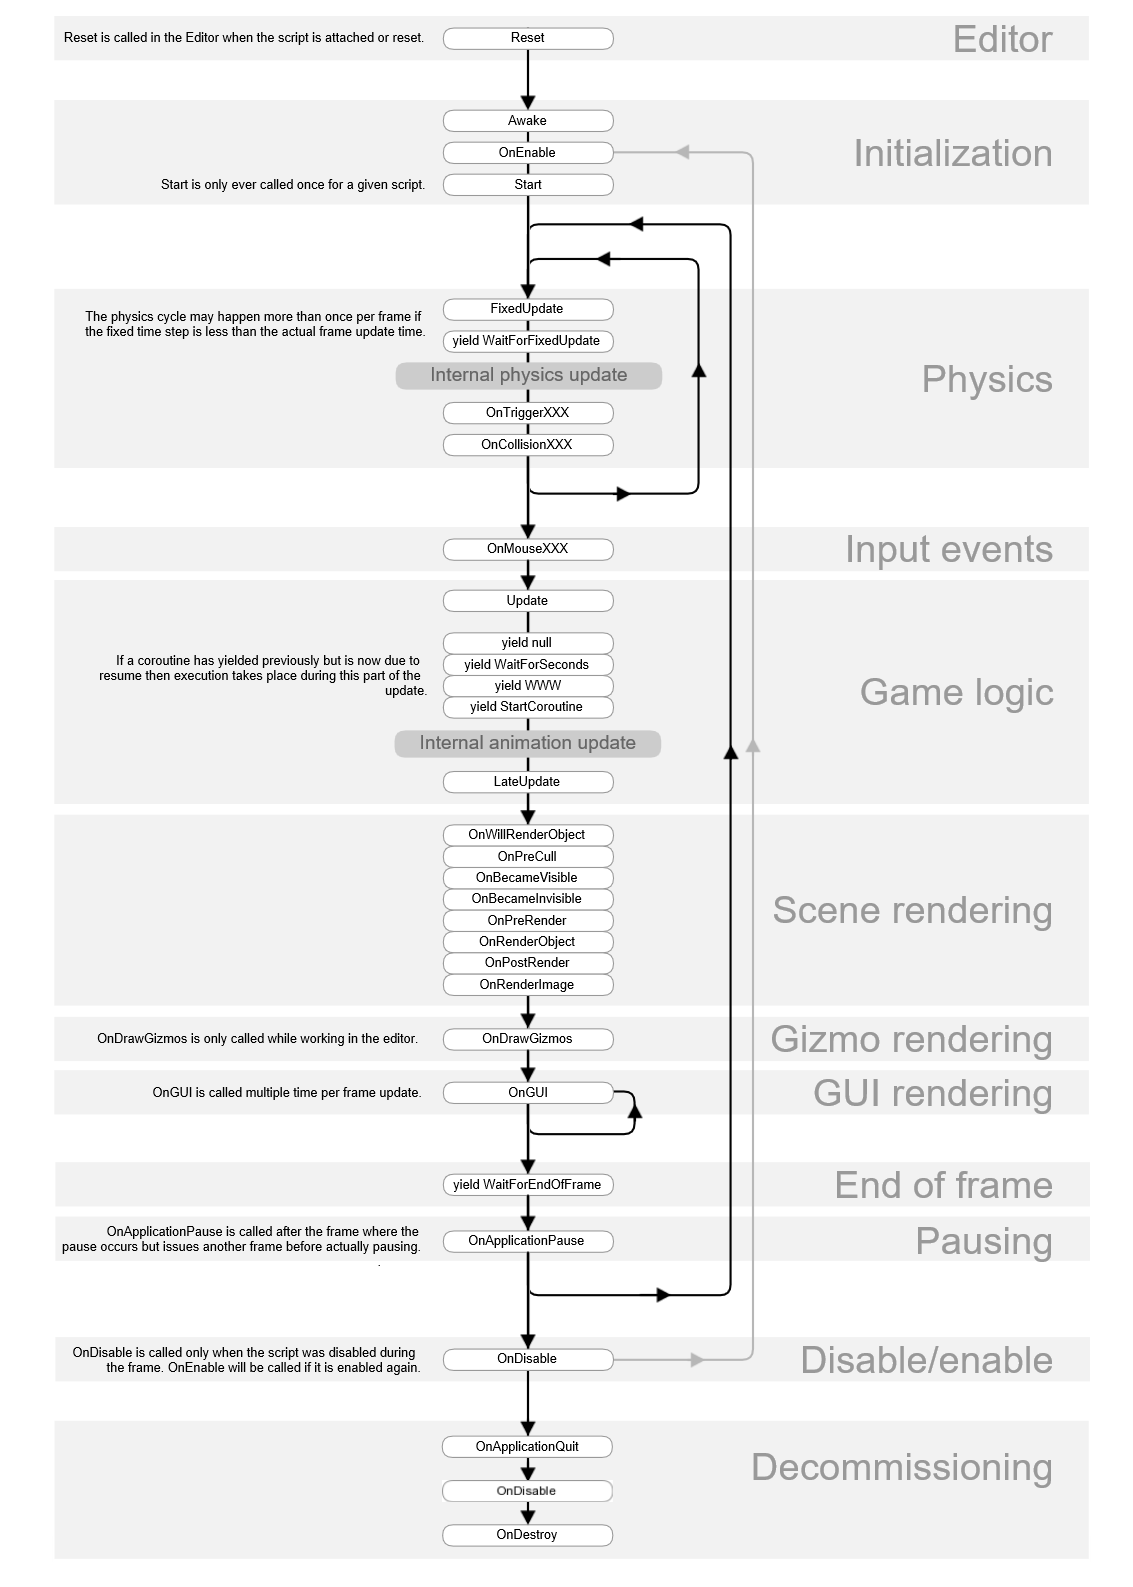
\includegraphics[width=1.0\textwidth]{Figs/monobehaviour_flowchart.png}
\caption{Script lifecycle flowchart with repetitions included \cite{Unity16}.}
\label{fig:monobehaviour} 
\end{figure} 

%********************************** %Second Section  **************************************
\section{\textit{Implementation details}} %Section - 4.2 

Molecule VR Viewer program consists of two scenes- menu and viewer scene- and each one contains the core script that manages all of the functionalities. In this section they are described in details.

\subsection{MainMenu.cs}

MainMenu script is attached to the Main Camera of Menu scene, where the two-dimensional UI (User's Interface) configured in Editor mode, is presented (Figure \ref{fig:mainmenu}). Each UI element has its reference in the script, what enables pulling the data out of it. 

Start function is responsible only for adding the listener to the "Start" button, which is the ButtonFunction method. It it responsible for setting of the feedback message and checking the correctness of entered PDB ID Code, which means its length (PDB codes always have 4 characters) and its actual existence in PDB data base. The latter is done with the HttpWebRequest and HttpWebResponse classes from System.Net library. If the URL address responses, the Viewer scene is loaded with \textit{Unity's} SceneManager. If not, and the WebException occurs, method displays the WebException message on the feedback message presented to the user.

The Update function contains elements responsible for assigning the data inserted by the user and for changing the set of colouring styles depending on which drawing style was chosen. Variables, which are obtained from UI, are held by the Configurator class.

\subsubsection{Configurator.cs}

This class, which does not inherits from MonoBehaviour, initialises four static variables, which are pdbID, hideHydrogens, representationStyle and colouring, with corresponding get and set methods. 

As the user's settings are needed during the entire gameplay, they need to be passed between scenes, which is more challenging than, e.g. communication between objects. The GameObject, where they are set, is no longer needed, therefore using the \textit{Unity's} method DontDestroyOnLoad, which prevents the object from being trashed while loading another scene, is not the best solution. This is why the other way was chosen, which is the usage of static attributes, that are available as long as the application is running. 

\subsection{MoleculeViewer.cs}

Viewer scene, which is loaded after successful request from the PDB server, is managed by the MoleculeViewer script, which constitutes the core of the whole program. It is the only component (except, obviously, Transform component) attached to the GameObject called CameraParent. The reason of that setting is explained later in this section.

In this case, Start function contains all the components needed for creation of structure representation in a way chosen by the user in main menu. First of all, the object of the FileReader class is initialized and its method ReadFile is called.

\subsubsection{FileReader.cs}

This class does not inherit from MonoBehaviour and provides the engine for extracting needed data from PDB database. Therefore, at the very beginning it downloads the PDB file and reads it line by line.

This is a good moment to introduce and describe the PDB file format. Its main property is its linearity- the content is presented in number of lines, with 80 columns per each. First six columns contain a record name, which defines the record type of the line. This is a very useful feature, as every record type is divided into fields, that have standardised positions in the line. Knowing the exact location of interesting data is very convenient in terms of file analysis. Because PDB file may contain a large variety of record types, only those, that were used in this work, are described below \cite{PDB16}.

\begin{itemize}
\item COMPND– macromolecular contents of an entry presented in a form of specification list. Specifications that were used in Molecule VR Viewer are MOLECULE, where the macromolecule name is defined, and CHAIN, which provide list of subunits identifiers, separated by commas.
\item SEQRES– listing of the linearly linked chemical components that form a polymer. For proteins these are amino acids, presented in a form of three-letter codes, and for nucleic acids- their residues. 
\item ATOM- atomic coordinates of an atom that belongs to a standard residue, its name, element symbol, serial number, occupancy, temperature factor, charge and belonging to subunit and residue. XYZ coordinates are in Angstroms. What is important, these records are listed in an ordered way, for proteins from amino to carboxyl terminus, and for nucleic acids- from the 5' to the 3' terminus.
\item HETATM- atomic coordinates of an atom that does not belong to the polymer, its name, element symbol, serial number occupancy, temperature factor, charge and belonging to subunit and residue. Useful especially for prosthetic groups, inhibitors, solvent molecules, metal ions etc.
\item CONECT- specifies connectivity between atoms, mostly for non-standard atoms and disulfide bridges, by assigning to the atom's serial number all the atoms that are bonded with it. 
\item HELIX- specifies the position of helices in a molecule by indication of the initial and ending residue. Helix type is also described by the number corresponding with helix class.
\item SHEET- specifies the position of sheets in a molecule similarly as in HELIX.
\end{itemize}


%\lstset{style=sharpc}
%\begin{lstlisting}
%MonoBehaviour
%\end{lstlisting} 







\nomenclature[z-IDE]{IDE}{Integrated Development Environment}
\nomenclature[z-UI]{UI}{User's Interface}